\chapter{Differential Equation Model}
\label{chapter:diffeq}

In this chapter we present a longitudinal analysis performed on the DRC data using the differential equation model (see section \ref{sec:dem}). In section \ref{sec:demClinicalQuestions} we present the clinical questions that we want to answer, in section \ref{sec:demMethod} we present the methodological details, in \ref{sec:demResults} we present the results and in \ref{sec:demDiscussion} we discuss our findings. 

% \section{Background}

% Summarise what has been reported so far in the literature
%TODO

\section{Clinical questions}
\label{sec:demClinicalQuestions}

The main questions we want to answer in this longitudinal analysis are:
\begin{enumerate}
\item In PCA, what are the differences in timing of atrophy and rates of atrophy between different brain regions? 
\item In tAD, what are the differences in timing of atrophy and rates of atrophy between different brain regions? 
\item Do people with PCA and AD lose brain volume at same speed? 
\item What are the differences in rates of atrophy across brain regions in PCA compared to AD? 
\end{enumerate}

\section{Method}
\label{sec:demMethod}

We used the differential equation model as described in section \ref{sec:dem}, where we fit a Gaussian Process (GP) to the change in biomarker scores $\Delta s / \Delta t$. The GP was fit independently for each biomarker. We used a non-parametric model such as GPs in order not to impose any parametric shape of the biomarker trajectory. Furthermore, given that the DRC dataset has a well-defined control population, we do not include the controls in the fitting of the GP as there is very little change in their biomarker values across timepoints which is not due to measurement noise. Moreover, in order to get a good fit of the GP we normalise the average biomarker values to z-scores and standardise the rates of change by dividing them with the average rate of change of all patients. The prior of the GP is kept at $Y=0$, which ensures that the trajectory has upper and lower asymptotes. 

After fitting the GP process we extracted the mean of the GP and sampled 20 trajectories from the posterior distribution of the GP in order to measure uncertainty in the model fit. The mean trajectory and trajectory samples were integrated using the numerical approach from Eq. \ref{eq:dem3}. The resulting trajectories were however not aligned on the temporal axis, since we fit the model for each biomarker independently. We therefore aligned the $t=0$ point so that $f(t=0)$ is the average biomarker value for every patient at baseline visit. More information about the alignment is give in section \ref{sec:demTrajAlignSimple}. This process was repeated independently for every mean trajectory in every biomarker. We also aligned the sampled trajectories in a similar fashion, with the only distinction that at the alignment point we added an amount of noise on the y-axis. This noise was computed as the standard deviation of the biomarker measurements for each patient at baseline visit. In order to discuss the differences in rates of atrophy across different biomarkers of diseases, we qualitatively compare the rates of atrophy at the point where the maximum rate of atrophy is attained. Moreover, a meaningful comparison of rates of atrophy across biomarkers requires them to be in a similar scale, so we converted the biomarker values representing ROI volumes to z-scores relative to controls. 

\section{Results}
\label{sec:demResults}

In Fig. \ref{fig:trajDEMPCA} we show the temporally aligned average trajectories for PCA subjects across several ROIs, while in Fig. \ref{fig:trajDEMAD} we show the trajectories for AD subjects. On the x-axis we show the number of years since baseline visit, while on the y-axis we show the z-score of the ROI volume relative to controls. The direction of the "ventricles" biomarker has been manually flipped for consistency with the other biomarkers. In Fig. \ref{trajDEMPcaAd} we show the trajectories of ROI volumes aligned for PCA and tAD along with integrated samples from the GP posterior that have been integrated and temporally aligned. The integrated posterior samples give an idea of the confidence in the average biomarker trajectory. Results from figure \ref{fig:trajDEM} can help us answer questions 1 and 2, while results from Fig. \ref{trajDEMPcaAd} can help us answer questions 3 and 4. 

\section{Discussion}
\label{sec:demDiscussion}

In the PCA progression from \ref{fig:trajDEMPCA}, in terms of timing of atrophy we find that the occipital and parietal lobes are the regions most affected early in the disease time course, before baseline visit. However, soon after baseline visit other biomarkers such as whole brain, temporal lobe and ventricles become abnormal. This matches our previous results on the same dataset using a fundamentally different model (the EBM, see section \ref{ebm:pca}), but provides more detail on the exact timing of atrophy. In terms of rates of atrophy, we see that the whole brain, ventricles and the temporal lobe are the ones showing the highest drop, which happens between baseline visit and 5 years later. While these findings confirm previous results in the literature \cite{lehmann2011cortical,whitwell2007imaging}, they provide a more detail regarding the exact timing and rate of atrophy decline over a timespan of 30 years. 

In the tAD progression from \ref{fig:trajDEMPCA}, in terms of timing of atrophy we find that the hippocampus is the first to become abnormal in the early stages, which is something that has been consistently confirmed across many other studies. Our model also predicts that in early stages the hippocampus is more sensitive than the entorhinal cortex and that the hippocampal atrophy precedes entorhinal atrophy. This has been confirmed by some previous studies \cite{laakso2000hippocampus,fonteijn2012event} but rejected by others \cite{braak1994morphological,pennanen2004hippocampus}. However, in middle and late stages we see a much more global patterns of atrophy affecting most brain areas. In terms of rate of atrophy, we find that in early stages many regions have a similar rate of decline, with only the hippocampus and ventricles showing a slightly slower rate. This is in contrast with previous findings in the literature such as \cite{scahill2002mapping} that find the hippocampus to have the highest rate of decline. We also find very similar rates especially right after the baseline visit, with slightly higher drops in volume for temporal and whole brain biomarkers.

When comparing PCA versus tAD, we find several differences in atrophy timings, rates and extent. In terms of whole brain, there is a comparable timing and rate of atrophy in both PCA and tAD in early stages, but in later stages at around baseline we find that there is more atrophy in PCA as compared to tAD. For the ROIs, we find that in PCA there is a significant amount of early and extensive atrophy in occipital and parietal areas as compared to tAD. On the other hand, in tAD there is significantly more atrophy in the hippocampus and entorhinal areas at any point in the disease, with more extensive atrophy in the hippocampus. Moreover, the hippocampus also reaches abnormal levels (-1 standard deviation) much earlier (15 to 10 years before baseline scan) in tAD compared with PCA (2 to 3 years after baseline scan). We notice that for many biomarkers sch as temporal, entorhinal and frontal there are reasonably similar rates of atrophy at many stages of the two diseases. 

\begin{figure}
\begin{subfigure}{\textwidth}
 \centering
%  \hspace{-2.5cm}
 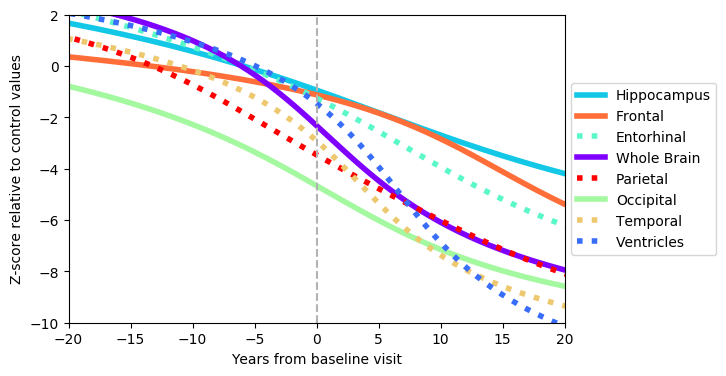
\includegraphics[scale=0.5]{images/dem/mriSmallSebPaper_DEMStdPCA_trajAlign.png}
 \caption{PCA progression}
 \label{fig:trajDEMPCA}
\end{subfigure}
\begin{subfigure}{\textwidth}
 \centering
%  \hspace{-2.5cm}
 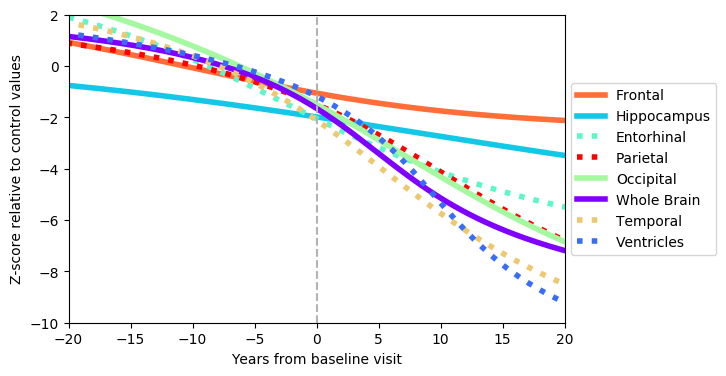
\includegraphics[scale=0.5]{images/dem/mriSmallSebPaper_DEMStdAD_trajAlign.png}
 \caption{tAD progression}
  \label{fig:trajDEMAD}
\end{subfigure}
\caption{Trajectories of different ROI volumes from the differential equation model on the (a) PCA progression and (b) tAD progression. On the x-axis we show the number of years since baseline visit, while on the y-axis we show the z-score of the ROI volume relative to controls.}
\label{fig:trajDEM}
\end{figure}

\begin{figure}
 \centering
%  \hspace{-3em}
 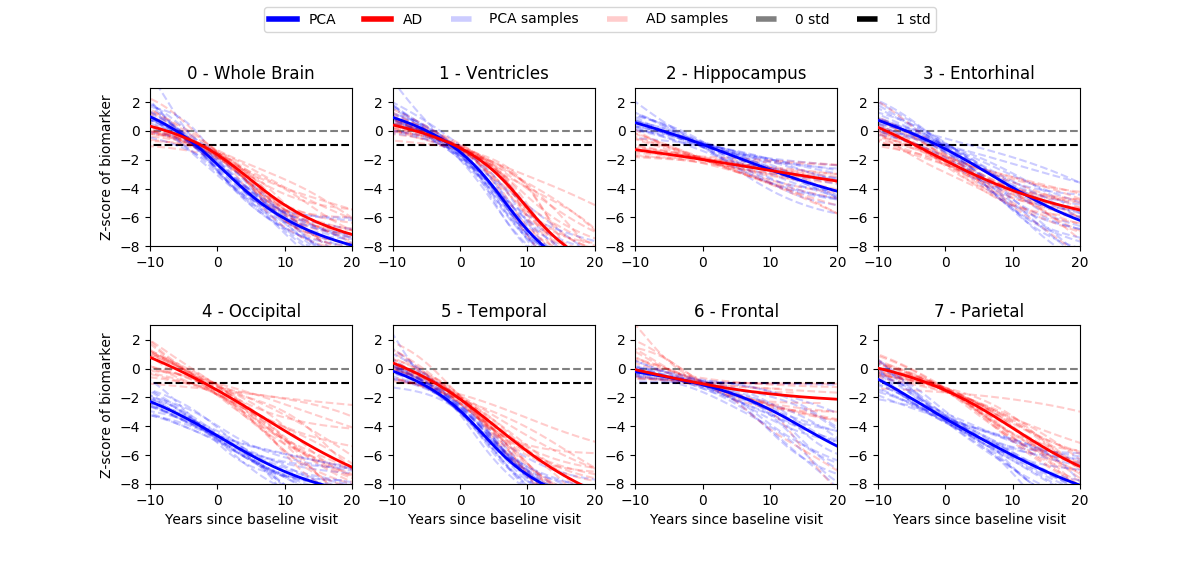
\includegraphics[scale=0.6,trim=100 0 100 0]{images/dem/mriSmallSebPaper_DEMStd_subplotsPcaAd.png}
 \caption{Mean trajectories of ROI volumes for PCA and tAD aligned on the same temporal scale along with samples from the posterior distribution showing the confidence in the mean trajectory. On the x-axis we show the number of years since baseline visit, while on the y-axis we show the z-score of the ROI volume relative to controls.}
 \label{trajDEMPcaAd}
\end{figure}

\section{Conclusion}
\label{sec:demConclusion}

% Summary
In this section we presented a longitudinal analysis of volume changes in PCA and tAD using the differential equation model. We compared the timing, rates and extent of atrophy across different regions in both PCA and tAD. Moreover, we also compared the evolution of each of these biomarkers across the two AD subtypes: tAD and PCA. While the patterns of tAD progression have been extensively studies using MRI biomarkers, there is significantly less literature on the progression of PCA. This analysis is the first to use data-driven disease progression models for studying atrophy evolution in PCA. Our analysis is also the first to directly compare MRI biomarkers in PCA vs tAD in terms of timing, rate and atrophy extent. 

% Limitations
There are several limitations with our analysis. First of all, we aligned the trajectories using the average biomarker value at patient baseline visit. This makes the assumption that the biomarker values corresponding to the stages of each patient at baseline only change linearly in that region. Secondly, the model fits each biomarker trajectory independently from the others and doesn't model biomarker correlations. Third, the confidence given by the posterior samples is not a true confidence interval, because these samples also have to be temporally aligned. This can bias the confidence interval, in making it smaller near the alignment point and larger at the ends. Moreover, the time $t=0$ is set as the time since baseline scan instead of disease onset. This becomes problematic when comparing across different diseases (PCA vs tAD) as symptoms might develop at different stages in the disease and this will influence when the subjects will come to the clinic for a baseline scan and assessment. 

% Future work drawing from the limitations
There are several possibilities for future work. The model can be extended to a multimodal framework by fitting an N-dimensional GP on the data and then integrating along all the biomarker values at the same time. This extension will remove the need to align the trajectories from different biomarker on the same temporal axis, but one still needs to set a $t=0$ starting point. Other clinical questions should also be explored, such as analysing subgroups within PCA, performing time to symptom onset analyses or asymmetry analyses. Other types of MRI biomarker measurements such as cortical thickness should also be analysed and linked to cognitive measures. 
